%%%%%%%%%%%%%%%%%%%% BEGIN GRAV %%%%%%%%%%%%%%%%%
\section{Movimiento planetario}

Uno de los problemas fundamentales del pensamiento del hombre en la antigüedad, fue el movimiento de los cuerpos celestes. Este pensamiento impulsó el desarrollo de la ciencia hasta nuestros días. Inicialmente para explicar el movimiento de las estrellas errantes y de las estrellas fijas en el cielo, se desarrollaron los siguientes modelos planetarios. 

\subsection{Modelos planetarios}

\begin{enumerate}
\item \textbf{Modelo geocéntrico:} Este primer modelo fue formulado en el año $100$ por el astrónomo griego Ptolomeo de Alejandría. En este sistema la tierra era el centro del universo y el conjunto de las estrellas fijas inundaban el universo circundante alrededor de la tierra. Por otro lado, se asumió que las estrellas errantes que se observaban en la noches giraban en torno a la tierra, algunas describiendo trayectorias muy complicadas, conocidas como epiciclos~\cite{alonso-z}. Cabe anotar que este modelo tenía como fundamentación al ``hombre como el centro del universo'', fue apoyado fuertemene por la iglesia y prevaleció por alrededor de 1400 años.

\item \textbf{Modelo heliocéntrico:} Este modelo fue propuesto por el astrónomo polaco Nicolás Copérnico ($1473-1543$). Tiene como fundamentación al sol como el centro del universo.
Cabe anotar que la idea de tener al sol como centro del universo, no era una idea nueva. Se tienen datos históricos que argumentan que fue realmente una idea del filósofo Aristarco de Samos, muchos años atrás~\cite{alonso-z}.
\end{enumerate}

Cabe mencionar que los dos modelos anteriores lograron explicar el movieminto de las estrellas de una manera aceptable. Sin embargo, prevalecian algunos detalles que necesitaron un estudio y una compresion más profunda de los mismos. Pasados unos años, el físico Johanes Kepler ($1571-1630$) usó el modelo de Copérnico y descubrió las leyes planetarias después de hacer un cuidadoso análisis de los datos coleccionados por el astrónomo danes Tycho Brahe ($1546-1601$). Éste último murió sin poder dar una buena interpretación de sus datos, coleccionados durante toda su vida.
No obstante, estas leyes fueron empíricas y su explicación teórica fue dada unos años después por el Físico británico Isacc Newton ($1642-1727$). Este último hizo la contribución más notable a la dinámica de los cuerpos celestes, que hoy en día conocemos como la ley de la gravitación universal, formulada en el año $1686$ y publicada en el año de $1687$ en el famoso libro; ``Los Principia" (Philosophiae Naturalis Mathematica~\cite{Whitehead:268025}).



%%%%%%%%%%%%%%%%%%%%%%%%%%%%%%%%%%%%%%%%%%%%%%%%%%%%%%%
\subsection{Leyes de Kepler}

\begin{enumerate}
\item \textbf{LEY $1$}: Todos los planetas se mueven en órbitas elípticas con el sol en una de sus focos (ver Fig.~\ref{fig:ley1}).
%%%%%%%%%%%%%%%%
\begin{figure}[h]
\begin{center}
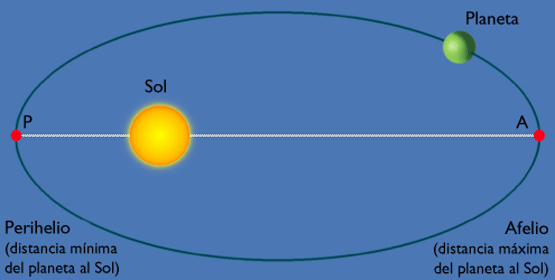
\includegraphics[scale=0.4]{gravitacion/g-ley1}
\end{center}
\caption{Primera ley de Kepler.}
\label{fig:ley1}
\end{figure}
%%%%%%%%%%%%%%%

Dicha ley generó una gran controversia para la época, debido a que las órbitas propuestas por el modelo heliocéntrico de Copérnico eran circulares y reflejaban la perfección del cielo. Las órbitas elípticas habían obstaculizado el trabajo Tycho Brahe durante toda su vida.
Cabe anotar que esta ley fue empírica. Fue deducida de la observación astronómica. Sin embargo, es un resultado de las estructura funcional de la fuerza de gravitación universal, la cual estudiaremos posteriormente.

\item \textbf{LEY $2$}: El radio-vector dirigido desde el sol a un planeta, barre áreas iguales en tiempos iguales (ver Fig.~\ref{fig:ley2}).
%%%%%%%%%%%%%%%%%
\begin{figure}[h]
\begin{center}
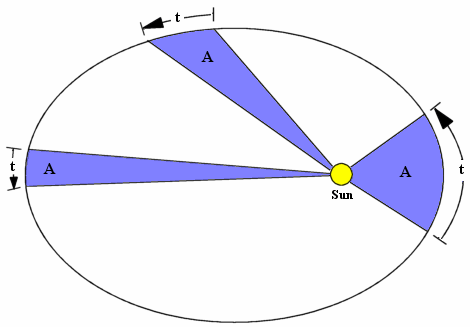
\includegraphics[scale=0.4]{gravitacion/g-ley2}
\end{center}
\caption{Segunda ley de Kepler.}
\label{fig:ley2}
\end{figure}
%%%%%%%%%%%%%%%%

Kepler obtuvo dicha ley estudiando detenidamente los datos obtenido en las observaciones astronómicas de Tycho Brahe. En la Fig.~\ref{fig:ley2} podemos ver que el área barrida en un tiempo $t$ fijo, siempre es $A$. 

Veamos las primeras implicaciones de esta ley. Supongamos que un planeta de masa $m$ está en órbita elíptica alrededor del sol. Consideremos un diferencial de área $dA$, tal como se muestra en la Fig.~\ref{fig:dA}.
%%%%%%%%%%%%%%%%%
\begin{figure}[h]
\begin{center}
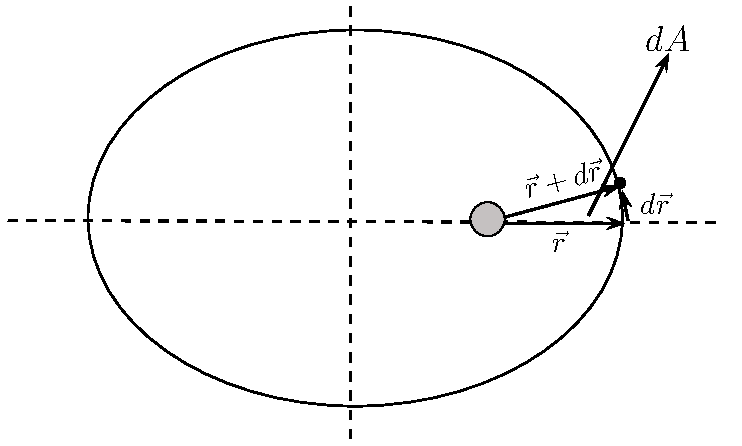
\includegraphics[scale=0.7]{gravitacion/g-dA}
\end{center}
\caption{Diferencial de área.}
\label{fig:dA}
\end{figure}
%%%%%%%%%%%%%%%%
\begin{equation}
dA = \dfrac{|\vec{r} \times d\vec{r}|}{2} 
\Rightarrow \dfrac{dA}{dt} = \dfrac{1}{2m}|\vec{r} \times m \dfrac{d\vec{r}}{dt}| = \dfrac{1}{2m}|\vec{r}\times \vec{p}|=\dfrac{|\vec{L}|}{2m}\,,
\label{ec:dA}
\end{equation}
donde $\vec{p}$ y $\vec{L}$ son el momento lineal y angular de la masa.
Así, de la ec.~\ref{ec:dA} queda claro que el hecho de que se barran áreas iguales en tiempos iguales tiene como consecuencia que el momento angular $\vec{L}$ de los planetas alrededor del sol es constante, es decir:
\begin{equation}
\vec{L}=\vec{r}\times \vec{p}=\vec{cte}\,.
\end{equation}
Además, esto establece uno de los precedentes fundamentales para la formulación de la ley de la gravitación universal. El hecho de que el momento angular sea una constante implica que la fuerza que está actuando sobre los planetas, es una fuerza central. Esto puede verse de la siguiente forma:
\begin{equation}
\vec{L}=\vec{r} \times \vec{p} \Rightarrow \dfrac{d\vec{L}}{dt}=\dfrac{d}{dt}(\vec{r}\times \vec{p}) =\dfrac{d\vec{r}}{dt}\times \vec{p} + \vec{r} \times \dfrac{d\vec{p}}{dt} = \vec{r} \times \dfrac{d\vec{p}}{dt}\,.
\label{ec:L-constante}
\end{equation}
Por lo tanto, el torque neto $\vec{\tau}$ que actúa sobre cada planeta, debido a su interacción con el sol, está dado por:
\begin{equation}
\vec{\tau}= \dfrac{d\vec{L}}{dt}= \vec{r}\times \dfrac{d\vec{p}}{dt} = \vec{r} \times \vec{F}\,,
\end{equation}
donde $\vec{F}$ es la fuerza neta que actúa sobre cada planeta. Ahora, si $\vec{L}$ es una constante, entonces la ecuación anterior implica que $\vec{r}\times \vec{F}= \vec{0}$, y por lo tanto $\vec{F}$ y $\vec{r}$ son antiparalelas (fuerza atractiva), es decir, \textit{la fuerza que mantiene en órbita a los planetas alrededor del sol, es una fuerza central atractiva}.\footnote{La fuerza $\vec{F}$ y el vector posición $\vec{r}$ no puden ser paralelos dado que la trayectoria es una curva cerrada.}

De lo anterior, tenemos que si consideramos dos puntos $p_1$ y $p_2$ sobre la trayectoria elíptica de cada planeta, se cumple que:
\begin{equation}
\vec{L}=\vec{cte} \Rightarrow |\vec{r}_1 \times \vec{p}_1 |=|\vec{r}_2 \times \vec{p}_2 | \Rightarrow |\vec{r}_1 \times m\vec{v}_1 |=|\vec{r}_2 \times m\vec{v}_2 |\,. \nonumber
\end{equation}
\begin{equation}
\Rightarrow|\vec{r}_1 \times \vec{v}_1 |=|\vec{r}_2 \times \vec{v}_2 |.
\end{equation}
%%%%%%%%%%%%%%%%%
\begin{figure}[h]
\begin{center}
\includegraphics[scale=0.8]{gravitacion/g-perihelio}
\end{center}
\caption{Perihelio y afelio de los planetas.}
\label{fig:relacion-vr}
\end{figure}
%%%%%%%%%%%%%%%%
En el caso particular del perihelio y el afelio  mostrado en la Fig.~\ref{fig:relacion-vr}:
\begin{equation}
|\vec{r}_1 \times \vec{v}_1 |=|\vec{r}_2 \times \vec{v}_2 |\Rightarrow v_1r_1 =v_2r_2 \Rightarrow 
\boxed{\dfrac{v_1}{v_2}=\dfrac{r_2}{r_1}}\,.
\end{equation}
De la ecuación anterior se puede inferir claramente que la rapidez de los planetas al pasar cerca al punto más cercano al sol, debe ser mayor a la rapidez que tengan dichos planetas cuando pasan por el punto más alejado del sol, es decir, la rapidez en el perihelio es mayor a la rapidez en el afelio.

\item \textbf{LEY $3$:} El cuadrado del periodo orbital $P$ de cualquier planeta es proporcional al cubo del semieje mayor $a$ de la órbita elíptica.

De acuerdo a la Fig.~\ref{fig:relacion-vr}:

\begin{equation}
P^2= k a^3 ,
\end{equation}

donde $k$ es una constante a determinar.

\end{enumerate}











%%%%%%%%%%%%%%%%%%%%%%%%%%%%%%%%%%%%%%%%%%%%%%%%%%%%%%%%%%%%%%%%%%
\section{Ley de Gravitación Universal}

En $1688$ Isaac Newton logró establecer con ayuda de las leyes de Kepler, la ley que gobierna el movimiento celeste de los cuerpos. Newton determinó que \textbf{cada partícula del universo atrae a los demás partículas del universo con una fuerza que es directamente proporcional al producto de sus masas e inversamente proporcional al cuadrado de la separación entre dichas masas}.

\begin{figure}[h]
\begin{center}
\includegraphics[scale=0.9]{gravitacion/fuerzagravitacional}
\end{center}
\label{fuerzagravitacional}
\caption{Fuerza de interacción gravitacional}
\end{figure}

Supongamos que tenemos dos partículas ``puntuales'' cuya separación es $r$, entonces, la fuerza que siente la partícula de masa $m_1$ debido a la partícula de masa $m_2$ es:

\begin{equation}
\boxed{
\vec{F}_{12}= G \dfrac{m_1m_2}{r^2}\hat{u}_r = -\vec{F}_{21}
} 
\end{equation}

donde $G$ es conocida como la constante gravitacional; $G=6.673 \times 10^{-11}$ Nm$^2$/kg$^2$. Note que $\vec{F}_{12}$ y $\vec{F}_{21}$ forman un \textbf{par acción-reacción} y además son fuerzas atractivas.



\subsection{Ejemplos:}

\begin{enumerate}

%ejercicio1
\item Ley de kepler para un MCU





%%%%%%%%%%%%%%%%%%%%%%%%% EJEMPLO 2 %%%%%%%%%%%%%%%%%%%%%%%%%%%%%%%%%%%
\vspace{0.5 cm}
%ejercicio2
\item Dos estrellas de masas $m$ y $M$ separadas por una distancia $d$, giran en  órbita circular alrededor de su centro de masa CM, tal como se muestra en la parte izquierda de la Fig.~\ref{fig:sistema-binario-Mm}. 
%
\begin{figure}[h]
\begin{center}
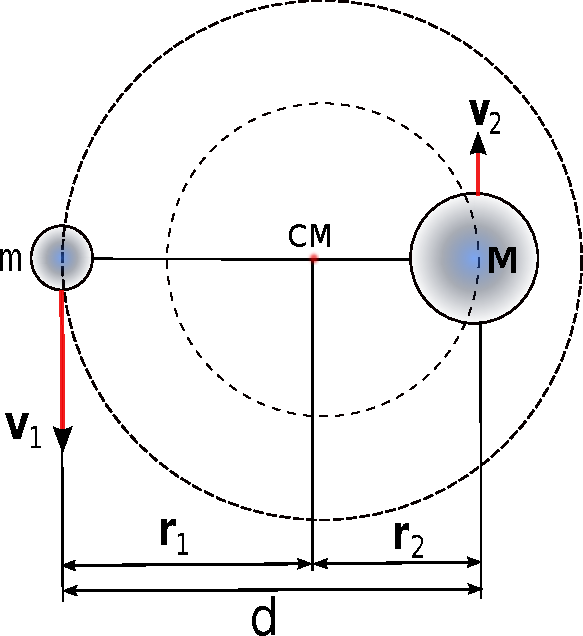
\includegraphics[scale=0.6]{gravitacion/sistema-binario-Mm}\hspace{1.0 cm}
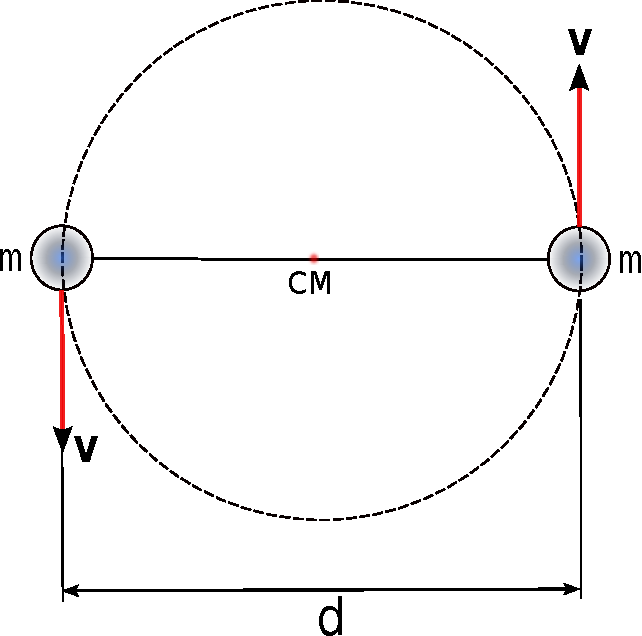
\includegraphics[scale=0.6]{gravitacion/sistema-binario-mm}
\end{center}
\caption{Sistema binario de estrellas en órbitas circulares con distintas e iguales masa.}
\label{fig:sistema-binario-Mm}
\end{figure}
%
\begin{enumerate}
\item Determinar el periodo de cada estrella.
\item Suponga que $M\gg m$. En este caso, se puede asumir que la masa $M$ está en el centro de masa del sistema. 
¿Cuál es el periodo en este caso? ¿Es compatible con la tercera Ley de Kepler para el movimiento elíptico con excentricidad 0 (órbita circular)?
%
\item El sistema binario Plaskett consiste de dos estrellas de masas iguales girando en torno a su centro de masa CM, tal como se muestra en la parte derecha de la Fig.~\ref{fig:sistema-binario-Mm}. 
La rapidez de cada estrella es aproximadamente $v = 300$ km/s y el periodo orbital es de $14,396$ días~\url{https://en.wikipedia.org/wiki/Plaskett%27s_Star}. 
Use el resultado del primer literal para determinar la masa $m$ de cada estrella.
\end{enumerate}

Solución:
\begin{enumerate}

\item En primer lugar,  sabemos que la fuerza que experimenta la masa $M$ debido a su interacción con la masa $m$ esta dada por ley de gravitación universal:
%
\begin{align}
\label{ec1:LGU-eje2}
F=\,&G \dfrac{Mm}{d^2}
\end{align}

Por otro lado, sabemos que la fuerza gravitacional que actúa sobre las masas es de carácter central y que el movimiento alrededor de su centro de masa es circular uniforme con distintos radios $r_1$ y $r_2$, pero con igual velocidad angular $\omega$. 
Por lo tanto, la fuerza que experimenta la masa $M$ debido a su interacción con la masa $m$ está dada por:
%
\begin{align}
\label{ec2:LGU-eje2}
F=\,& M\dfrac{v_2^2}{r_2}=M\omega^2r_2\,.
\end{align}
%
Note que usamos la relación $v=\omega r$, para un movimiento circular uniforme. 

Análogamente, la fuerza central que experimenta la masa $m$ debido a su interacción con la masa $M$ está dada por la siguiente expresión:
%
\begin{align}
\label{ec3:LGU-eje2}
F=\,& m\dfrac{v_1^2}{r_1}=m\omega^2r_1\,.
\end{align}
%
Ahora, si multiplicamos la ec.~\eqref{ec2:LGU-eje2} la masa $m$ y la ec.~\eqref{ec3:LGU-eje2} la masa $M$ y las sumamos, tenemos la siguiente ecuación:
%
\begin{align}
\label{ec4:LGU-eje2}
F(m + M) =\,& \omega^2Mm\left(r_1+r_2\right)\,.
\end{align}
%
Despejando la fuerza $F$ de la ec.~\eqref{ec1:LGU-eje2} y reemplazando en la ec.~\eqref{ec4:LGU-eje2}, tenemos que:
%
\begin{align}
\label{ec5:LGU-eje2}
G\dfrac{Mm}{d^2}(m+M)=\,&\omega^2Mm\left(r_1+r_2\right)\,.
\end{align}
%
Finalmente, usamos la definición del periodo en un movimiento circular uniforme $P=\dfrac{2\pi}{\omega}$ y la relación $r_1+r_2=d$ mostrada en la Fig.~\ref{fig:sistema-binario-Mm}, para concluir que:
%
\begin{align}
\label{ec6:LGU-eje2}
P^2=\,&\dfrac{4\pi^2}{G(m+M)}d^3\,.
\end{align}

\item Si asumimos que $M\gg m$ en la ec.~\eqref{ec5:LGU-eje2}, entonces:
%
\begin{align}
\label{ec7:LGU-eje2}
P^2~\approx\,&\dfrac{4\pi^2}{GM}d^3\,,
\end{align}
es decir, obtenemos la tercera ley de Kepler para el caso de un movimiento circular. Recordemos que esta ley fue originalmente deducida para el sistema planetario en el cual la masa del sol es mucho mayor que la masa de los planetas, y en este contexto la aproximación $M\gg m$ es completamente válida. De igual forma, es importante aclarar, que las órbitas planetarias realmente son elípticas en las cuales la distancia $d$ debe ser interpretada como el semieje mayor de la elipse (parámetro comúnmente llamado $a$). Por lo tanto, podemos afirmar que este resultado es compatible con la tercera ley de Kepler.

\item Usando la ec.~\eqref{ec6:LGU-eje2} con $M=m$, tenemos que:
%
\begin{align}
\label{ec8:LGU-eje2}
m=\,&\dfrac{2\pi^2 d^3}{G P^2}\,,
\end{align}
%
además, en el movimiento circular se cumple que:
\begin{align}
\label{ec9:LGU-eje2}
P=\,&\dfrac{2\pi}{\omega}=\dfrac{2\pi R }{v}=\dfrac{\pi d}{v}\,,
\end{align}
donde usamos la relación $R=d/2$ entre el diámetro y el radio de la órbita circular.
Combinando las dos últimas ecuaciones tenemos que:
\begin{align}
m=\,&\dfrac{2v^3P}{\pi G} = \dfrac{2\times(3\times 10^5\, \text{m/s})^3\times ( 14.396 \times 24\times 3600\, \text{s})}{\pi\times 6,673\times 10^{-11} \text{Nm}^2/\text{kg}^2}
\approx 3.204\times 10 ^{32}\, \text{kg}\,,
\end{align}
%
es decir, alrededor de cien veces la masa del sol ($M_{\odot}\approx 1.988 \times 10^{30}\,\text{kg}$).
\end{enumerate} 





\vspace{0.5 cm}
%%%%%%%%%%%%%%%%%%%%%%%%% EJEMPLO 3 %%%%%%%%%%%%%%%%%%%%%%%%%%%%%%%%%%%
\item Suponga que un satélite de masa $m=2000$ kg está en órbita elíptica alrededor de la tierra.
En el perigeo (punto de mayor cercanía a la tierra) tiene una altitud de 1100 km y en el apogeo (punto de mayor lejanía a la tierra) tiene una altura de 4100 km. 
Suponga que se quiere transferir el satélite desde la órbita elíptica a la órbita circular 
cambiando su velocidad en el perigeo, tal como se muestra en la Fig.~\ref{fig:cambio-orbita}. 
Asuma que el radio terrestre es $R\approx 6400$ km. 
%
\begin{figure}[h]
\begin{center}
\includegraphics[scale=0.8]{gravitacion/cambio-de-orbita}
\end{center}
\caption{Cambio de órbita de un satélite.}
\label{fig:cambio-orbita}
\end{figure}
%
\begin{enumerate}
\item Determinar la energía mecánica del satélite en ambas órbitas.
\item Determinar la excentricidad de la órbita elíptica.
\item ¿Cuál debe ser el cambio en la velocidad del satélite en el perigeo para realizar la transferencia hacia la órbita circular?
\item Determinar el momento angular en ambas órbitas.
\end{enumerate}

Solución:
\begin{enumerate}
\item La energía mecánica de un cuerpo de masa $m$ en un órbita elíptica alrededor de un cuerpo de masa $M\gg m$ esta dada por la expresión:
%
\begin{align}
\label{ec1:eje3}
E=\,&-\dfrac{GmM}{2 a}\,,
\end{align}
%
donde $a$ es el semieje mayor de la órbita. 
Por lo tanto, la energía mecánica en la órbita elíptica es: 
%
\begin{align}
\label{ec2:eje3}
E_1=\;&-\dfrac{GmM}{2 a} = -\left(\dfrac{GM}{R^2}\right)\dfrac{mR^2}{2a}=-g\dfrac{mR^2}{2a}
\end{align}
%
donde $g=9.8\; \text{m}/\text{s}^2$ es la aceleración de la gravedad sobre la superficie terrestre. Reemplazando los valores numéricos:
%
\begin{align}
\label{ec3:eje3}
E_1=\;& -9.8\; \text{m}/\text{s}^2 \left(\dfrac{2\times 10^3 \text{kg}\times (6400\times 10^3 \text{m})^2}{\left(1100+4100+2(6400)\right)\times 10^3 \text{m}}\right)\approx -4.46 \times 10^{10} \text{J}\,.
\end{align}
%
Análogamente, en la órbita circular, la energía mecánica también está dada por la ec.~\eqref{ec1:eje3}, donde ahora el semieje mayor de la órbita debe ser interpretado como la distancia que hay al perigeo, es decir:
%
\begin{align}
\label{ec4:eje3}
E_2=\;& -9.8\; \text{m}/\text{s}^2 \left(\dfrac{2\times 10^3 \text{kg}\times (6400\times 10^3 \text{m})^2}{2\left(1100+6400\right)\times 10^3 \text{m}}\right)\approx -5.35 \times 10^{10} \text{J}\,.
\end{align}

\item La excentricidad de la órbita elíptica puede determinarse usando la expresión:
\begin{align}
\label{ec5:eje3}
\epsilon=\;& \dfrac{r_{\text{max}}-r_{\text{min}}}{r_{\text{max}}+r_{\text{min}}}\,,
\end{align}
%
donde $r_{\text{max}}$ y $r_{\text{min}}$ son respectivamente las distancias al apogeo y al perigeo de la órbita elíptica. Recuerde que estas son las distancias de mayor lejanía y mayor cercanía entre los centros de masa de ambos cuerpos. En este caso:
\begin{align}
\label{ec6:eje3}
\epsilon=\;& \dfrac{((R+4100)-(R+1100))\;\text{km}}{((R+4100)+(R+1100))\;\text{km}}=\dfrac{3000}{(2R+5200)}=\dfrac{3000}{12800+5200}=\dfrac{1}{6}\,.
\end{align}

\item Para determinar el cambio en la velocidad del satélite, calculemos primero su rapidez en el perigeo para cada una de las dos órbitas. En este punto esta rapidez es fija una vez se tiene una órbita de movimiento.
Para lo anterior, usaremos la definición de la energía mecánica para la órbita elíptica en el perigeo:
%
\begin{align}
\label{ec7:eje3}
E_1=&\;-G\dfrac{M\,m}{r_{\text{min}}}+\dfrac{1}{2}m\, v_1^2\,,
\end{align}
%
Por lo tanto:
%
\begin{align}
\label{ec8:eje3}
v_1=\sqrt{\dfrac{2}{m}\left(E_1+G\dfrac{m\,M}{r_{\text{min}}}\right)}
=\sqrt{\dfrac{2}{m}\left((E_1+g\dfrac{mR^2}{r_{\text{min}}}\right)}\,,
\end{align}
donde usamos nuevamente el valor de la gravedad sobre la superficie terrestre.
%
Finalmente, podemos concluir que el cambio en la rapidez está dado por:
\begin{align}
\label{ec9:eje3}
\Delta v =&\; (v_2-v_1)=\sqrt{\dfrac{2}{m}}\left[\sqrt{\left(E_1+g\dfrac{mR^2}{r_{\text{min}}}\right)}-\sqrt{\left(E_2+g\dfrac{mR^2}{r_{\text{min}}}\right)}\right]\approx -584.784\; \text{m/s} \,,
\end{align}
%
donde tuvimos en cuenta que la rapidez $v_2$ tiene la misma estructura de la ec.~\eqref{ec8:eje3} cambiando $E_1$ por la energía $E_2$. De este resultado se puede concluir que el satélite debe disminuir su velocidad para poder pasar desde la órbita elíptica a a la órbita circular.

\item El momento angular en ambas órbitas es respectivamente:
\begin{align}
L_1=&\; |\vec{r}_1\times \vec{p}_1|= m\, r_{\text{min}}v_1 \approx 1.18531\times10^{14}\; \text{kg m}^2/\text{s}\\
L_2=&\;|\vec{r}_2\times \vec{p}_2|= m\, r_{\text{min}}v_2 \approx 1.09759\times10^{14} \; \text{kg m}^2/\text{s}\,.
\end{align}


\end{enumerate}


















\end{enumerate}






\subsection{Ejercicios:}
\begin{enumerate}

\item Suponga que el movimiento de la tierra alrededor del sol es casi circular (la excentricidad $e$ de la órbita de la tierra es casi $0$) y determine la constante $k$ que aparece en la tercera ley del Kepler $P^2=ka^3$.

\item Calcule la masa el sol usando el periodo de rotación de la tierra alrededor del sol $P \approx 356$ días $\approx 3.156 \times 10^7$ s y sabiendo que la distancia tierra sol es $r \approx 1.496 \times 10^{11}$ m (distancia desde el centro de la tierra al centro del sol).

\item Calcule el valor de la gravedad terrestre usando el radio de la tierra $R\approx 6.37 \times 10^6$ m y la masa de la tierra $M \approx 5.98 \times 10^24$ kg.

\item Considere un satélite de masa $m$ que se mueve en órbita circular alrededor de la tierra con una rapidez $v$ constante y a una altura fija $h$ sobre la superficie terrestre. Si el satélite es geoestacionario (permanece en una posición fija sobre la tierra), ¿qué tan rápido debe moverse? y ¿a qué altura?\\
\textit{Respuesta:} $v=3.07 \times 10^3$ m/s, $h \approx 36000$ km.

\item Si el periodo de la luna alrededor de la tierra es de $28$ días, ¿cuál debe ser el periodo de un satélite que órbita la tierra a una distancia $1/10$ de la distancia tierra - luna?\\
\textit{Respuesta:} $T=28$ $(1/10^{3/2})$ días.

\end{enumerate}









%%%%%%%%%%%%%%%%%%%%%%%%%%%%%%%%%%%%%%%%%%%%%%%%%%%%%%%%%%
\section{Campo Gravitacional}

Supongamos que tenemos una masa puntual $m$ y a diferentes posiciones de $m$ ponemos una masa puntual $m'$. En cada posición $m$ experimenta una fuerza $\vec{F}$ debido a la atracción gravitacional.

\begin{figure}[h]
\begin{center}
\includegraphics[scale=0.8]{gravitacion/campo}
\label{campo}
\end{center}
\caption{Campo gravitacional generado por una masa puntual $m$}
\end{figure}

El campo gravitacional en un punto $P$ producido por la masa $m$ es definido como la fuerza ejercida sobre una unidad de masa $m'$ colocada en $P$, es decir, es la fuerza ejercida sobre una masa de prueba $m'$ dividida sobre $m'$, es decir:

\begin{equation}
\boxed{
\vec{g}_p(r)=\dfrac{\vec{F}}{m'}=-G\dfrac{m}{r^2}\hat{u}_r
}
\end{equation}     

Para el caso general de una distribución de masa volumétrica (Fig.~\ref{fig_distribucion_continuo} ), superficial o lineal; el campo gravitacional se calcula con la siguiente expresión:

\begin{equation}
\boxed{\vec{g}_p(r)=-G\int_M \dfrac{dm}{r^2}\hat{u}_r} ,
\label{ecucampogcontinuo}
\end{equation} 

donde la integral debe hacerse sobre todo el cuerpo de masa $M$. Note que que el la ecuación anterior, el vector unitario $\hat{u}_r$ y la magnitud $r$ son variables al igual que $dm$, tal como se muestra en la Fig.~\ref{fig_distribucion_continuo}. 

\begin{figure}[h]
\begin{center}
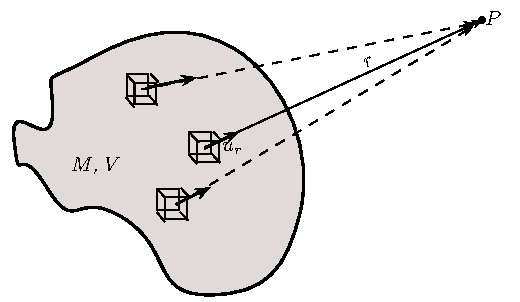
\includegraphics[scale=0.9]{gravitacion/figcampogcontinuo}
\caption{Campo gravitacional generado por una masa  $M$.}
\label{fig_distribucion_continuo}
\end{center}
\end{figure}







%%%%%%%%%%%%%%%%%%%%%%%%%%%%%%%%%%%%%%%%%%%%%%%%%%%%%%%%%%%%%%%%
\subsection{Energía potencial gravitacional $E_p(r)=U_p(r)$}

\begin{figure}[h]
\begin{center}
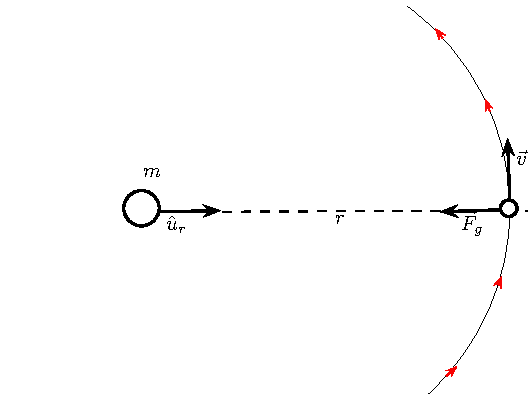
\includegraphics[scale=0.9]{gravitacion/energiapotencial}
\caption{Energía potencial}
\label{energia potencial}
\end{center}
\end{figure}

Dado que la fuerza gravitacional $\vec{F}_g$ es una fuerza central y sólo depende de la distancia $r$ entre las dos masas (Fig.~\ref{energia potencial} ), entonces $\vec{F}_g$ es una fuerza conservativa y podemos asociarle una función energía potencial gravitacional $E_p(r)$.

\begin{equation*}
\vec{F}_g(r)= -G\dfrac{mm'}{r^2}\hat{u}_r = -\vec{\nabla}E_p(r) = - \hat{u}_r \dfrac{\partial}{\partial r} E_p(r) 
\end{equation*}
\begin{equation*}
\Rightarrow -G \dfrac{mm'}{r^2}=- \dfrac{\partial}{\partial r} E_p(r) \Rightarrow \int _{\infty} ^{r} \dfrac{Gmm'}{r^2}dr = \int_{0}^{E_p} dE_p
\end{equation*}
\begin{equation}
\Rightarrow \boxed{E_p(r)= -\dfrac{Gmm'}{r}} ,
\label{energiag}
\end{equation}
donde hemos definido $E_p(\infty)=0$, es decir, hemos tomado el cero de energía potencial en el infinito.

Para un sistema de $n$ masas puntuales $m_1, m_2, \cdots, m_n$, la energía potencial del sistema está dada por:

\begin{equation}
E_p=U =\dfrac{1}{2}\sum_{i=1}^n\sum_{j=1\neq i}^n \dfrac{-Gm_im_j}{r_{ij}} = \sum_{j<i=1}^{n} \dfrac{-Gm_im_j}{r_{ij}} ,
\end{equation}

donde $r_{ij}$ es la magnitud del vector posición que va desde la masa $m_i$ hasta la masa $m_j$.\\

\subsection*{Ejemplos}

\begin{itemize}
\item Para dos masas puntuales $m_1$, $m_2$, separadas una distancia $r=r_{12}$:
\begin{equation}
U=-G \dfrac{m_1m_2}{r_{12}}=-G \dfrac{m_1m_2}{r}
\end{equation}
\item Para tres masas puntuales $m_1$, $m_2$, $m_3$, separadas distancias $r_{12}$, $r_{13}$, $r_{23}$ (ver Fig.~\ref{figtresmasas} para mayor ilustración):
\begin{eqnarray}
\nonumber
U&=&-G \dfrac{m_1m_2}{r_{12}}-G \dfrac{m_1m_3}{r_{13}}-G \dfrac{m_2m_3}{r_{23}} \\
&=&-G\bigg(\dfrac{m_1m_2}{r_{12}}+ \dfrac{m_1m_3}{r_{13}}+\dfrac{m_2m_3}{r_{23}})
\end{eqnarray}
\begin{figure}
\begin{center}
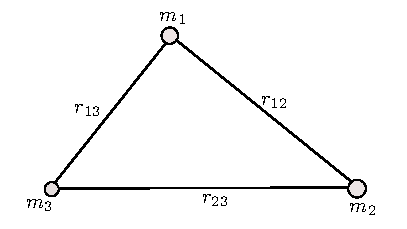
\includegraphics[scale=0.9]{gravitacion/tresmasas}
\end{center}
\caption{Tres masas puntuales}
\label{figtresmasas}
\end{figure}
\item Para cuatro masas puntuales $m_1$, $m_2$, $m_3$, $m_4$, separadas distancias $r_{12}$, $r_{13}$, $r_{14}$, $r_{23}$, $r_{24}$, $r_{34}$:
\begin{eqnarray}
\nonumber
U=-G\bigg(\dfrac{m_1m_2}{r_{12}}+ \dfrac{m_1m_3}{r_{13}}+\dfrac{m_1m_4}{r_{14}}+\dfrac{m_2m_3}{r_{23}}+\dfrac{m_2m_4}{r_{24}}+\dfrac{m_3m_4}{r_{34}}\bigg)
\end{eqnarray}
\end{itemize}

\subsection*{Ejemplo}
Un proyectil de masa $m$ es lanzado desde la superficie de la tierra formando un ángulo $\alpha$ con la vertical tal como se muestra en la Fig.~\ref{fig-tiro}. Si la rapidez inicial del proyectil es $v_0=\sqrt{\dfrac{GM}{R_e}}$, donde $M$ es la masa de la tierra, determinemos la altura máxima alcanzada por el proyectil (\textbf{$r_{max}$}).\cite{klepner} \cite{youngfisica}

\begin{figure}[h]
\begin{center}
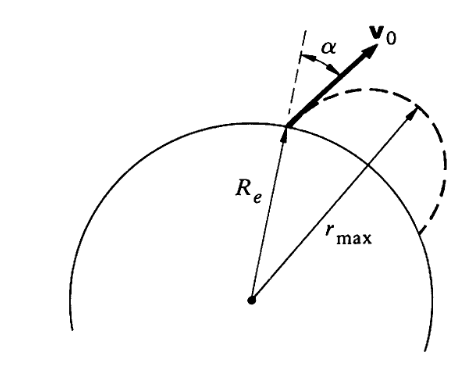
\includegraphics[scale=0.3]{gravitacion/tiro}
\end{center}
\caption{Altura máxima ($r_{max}$) en un tiro parabólico}
\label{fig-tiro}
\end{figure}

Usando la conservación de la energía mecánica del sistema masa-tierra, tenemos:
\begin{eqnarray}
\dfrac{1}{2}m v_{0}^{2} - \dfrac{GmM}{R}=\dfrac{1}{2}m v^{2} - \dfrac{GmM}{r_{max}},
\end{eqnarray}
donde $v$, es la rapidez cuando se alcanza la altura máxima.

Por otro lado, usando la conservación del momento angular del sistema masa-tierra, tenemos:
\begin{eqnarray}
mRv_{0}\sen{\alpha}=mr_{max}v
\end{eqnarray}
Usando las dos ecuaciones anteriores, tenemos que:
\begin{eqnarray}
r_{max}=R(1+\cos{\theta})
\end{eqnarray}










%%%%%%%%%%%%%%%%%%%%%%%%%%%%%%%%%%%%%%%%%%%%%%%%%%%%%%%%%
\subsection{Potencial gravitacional $V(r)$}

Se define el potencial gravitacional $V(r)$ como la energía potencial por unidad de masa $m'$ colocada en el campo gravitacional.
\begin{equation}
\boxed{V(r)=\dfrac{E_p(r)}{m'}= -\dfrac{Gm}{r}}
\end{equation}

Note que: 
\begin{displaymath}
g(r)=-\dfrac{Gm}{r^2}=-\dfrac{\partial}{\partial r}(-\dfrac{Gm}{r})
\end{displaymath}
\begin{equation}
\Rightarrow \boxed{ \vec{g}(r)= -\vec{\nabla}V(r) }
\label{gradienteg}
\end{equation}

La ecuación anterior es fundamental. El concepto de potencial gravitacional juega un papel muy importante en el cálculo de algunos campos, debido a que es una cantidad escalar, la cual ``casi'' siempre es más fácil de calcular que la cantidad vectorial $\vec{g}$. Una vez calculado $V(r)$ hallamos $\vec{g}$ usando la ec.~\eqref{gradienteg}. 

Definimos la \textbf{superficie equipontencial} como aquella superficie que rodea a la masa $m$ en la cual $V$ tiene el mismo valor.

\begin{figure}[h]
\begin{center}
\includegraphics[scale=0.8]{gravitacion/superficie}
\caption{Superficie equipotenciales de una carga puntual (curva a rayas).}
\label{superficie-equipotencial}
\end{center}
\end{figure}

Para el caso de distribuciones continuas de masa, el potencial gravitacional ha de calculase mediante la ecuación:

\begin{equation}
\boxed{V(r)= -G\int_M \dfrac{dm}{r}}
\end{equation}

\subsubsection{Principio de superposición para masas puntuales}

En cualquier campo $P$ (Fig.~\ref{camposuperposicion} ), el campo debido a un grupo de masas $m_1, m_2, \cdots, m_n$, es igual al vector suma de los campos $\vec{g}_i$ generados por cada una de masas individuales, es decir, el campo en el punto $P$ es la superposición de los campo individuales $\vec{g}_i$:

\begin{figure}[h]
\begin{center}
\includegraphics[scale=0.7]{gravitacion/camposuperposicion}
\end{center}
\caption{Principio de superposición para campos}
\label{camposuperposicion}
\end{figure}

\begin{equation}
\vec{g}=\sum_{i=1}^{n}\vec{g}_i = -\sum_{i=1}^{n}\dfrac{Gm_i}{r_i^2} \hat{u}_i
\end{equation}


Análogamente el potencial en el punto $P$ es:

\begin{equation}
V=\sum_{i=1}^{n}V_i = \sum_{i=1}^{n} \dfrac{-Gm_i}{r_i}
\end{equation}









%%%%%%%%%%%%%%%%%%%%%%%%%%%%%%%%%%%%%%%%%%%%%%%%%%%%%%%%%%%
\section{Movimiento general bajo interacción gravitacional}

Consideremos el movimiento de un cuerpo de masa $m$ alrededor de un cuerpo de masa $M>m$ tal como se muestra en la Fig.~\ref{fig:movimiento-general}.
%%%%%%%%%%%%%%
\begin{figure}
\begin{center}
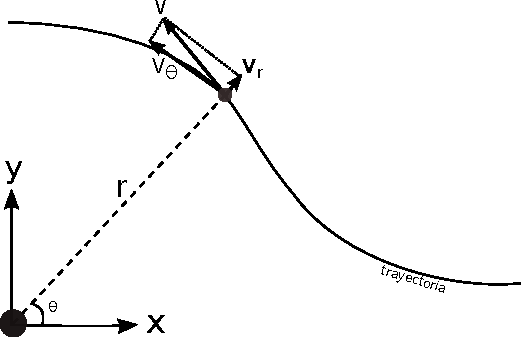
\includegraphics[scale=1]{gravitacion/g-movimiento-general}
\end{center}
\caption{Movimiento general de un cuerpo bajo interacción gravitacional.}
\label{fig:movimiento-general}
\end{figure}
%%%%%%%%%%%%
Según la conservación de la energía mecánica
\begin{align}
\label{eq:E-mecanica}
E =& \dfrac{1}{2}mv^2 + U(r) = \dfrac{1}{2}m(v_r^2+v_\theta^2) -\dfrac{G m}{r} = \dfrac{1}{2}m\left[\left(\dfrac{dr}{dt}\right)^2+\left(r\dfrac{d\theta}{dt}\right)^2\right] -\dfrac{G m}{r} \nonumber \\
=& \dfrac{1}{2}m\left(\dfrac{d\theta}{dt}\right)^2 \left[\left(\dfrac{dr}{d\theta}\right)^2+r^2\right]-\dfrac{G m}{r}\,.
\end{align}
%
Por otro lado, usando la definición de momento angular
\begin{align}
\label{eq:L}
\vec{L}=m\,\vec{r}\times\vec{v}=m\,\vec{r}\times(\vec{v_r}+\vec{v_\theta})= m\,\vec{r}\times\vec{v_\theta} \to L = m\,r \left(r\dfrac{d\theta}{dt}\right)\,.
\end{align}
Reemplazando la ec.~\eqref{eq:L} en la ec.~\eqref{eq:E-mecanica} tenemos que:
\begin{align}
\label{eq:drdthetat}
\left(\dfrac{dr}{d\theta}\right)^2 = \dfrac{m^2r^4}{L^2}\left(\dfrac{2E}{m}+\dfrac{2GM}{r}-\dfrac{L^2}{m^2r^2}\right)\,.
\end{align}

Por otro lado, en el estudio de la geometría se tiene que la ecuación de las cónicas es
\begin{equation}
\label{eq:conicas}
\dfrac{\epsilon d}{r} = 1 +\epsilon\cos\theta\,,
\end{equation}
donde $\epsilon$ es la excentricidad de la cónica, $d$ es la distancia a la directriz y $r,\theta$ son la coordenadas polares~\cite{alonso1967fundamental}.
Usando esta ecuación se tiene que
\begin{equation}
\label{eq:conica-drdtheta}
\left(\dfrac{dr}{d\theta}\right)^2=\dfrac{r^4\sin\theta^2}{d^2}\,.
\end{equation}
Por lo tanto, de acuerdo a las ecs.~\eqref{eq:drdthetat} y~\eqref{eq:conica-drdtheta} tenemos que:
\begin{align}
\sin\theta^2 =& \dfrac{d^2m^2}{L^2}\left(\dfrac{2E}{m}+\dfrac{2Gm}{r}-\dfrac{L^2}{m^2r^2}\right)=\left(1-\dfrac{d^2}{r^2}+\dfrac{2d}{r\epsilon}-\dfrac{1}{\epsilon^2}\right)\,,
\end{align} 
donde usamos la ec.~\eqref{eq:conicas}. Comparando las potencias en la coordenada $r$ tenemos las siguientes dos relaciones: 
\begin{itemize}
\item Potencias de $r^0$:
\begin{equation}
\label{eq:Energia-general}
1-\dfrac{1}{\epsilon^2}=\dfrac{2d^2mE}{L^2} \to E=\dfrac{L^2}{2d^2m}\left(1-\dfrac{1}{\epsilon^2}\right)\,.
\end{equation}
\item Potencias de $r^{-1}$:
\begin{equation}
\label{e:excentricidad}
\dfrac{2d}{r\epsilon}=\dfrac{2d^2m^2GM}{rL^2} \to \epsilon=\dfrac{L^2}{dm^2GM}\,.
\end{equation}
\end{itemize}

A continuación, en la Tabla~\ref{tab:conicas-interpretacion}. mostramos algunas características de las tres cónicas mostradas, enfatizando en el caso particular de la elipse. 
%%%%%%%%%%%%%
\begin{table}[h]
\begin{center}
\begin{tabular}{|c|c|c|c|}
\hline
Cónica & Excentricidad & Energía & Momento angular \\
\hline
&&&\\
Elipse & $0\leq\epsilon<1$ & $E=-\dfrac{GMm}{2a} < 0$& $L^2=Gm^2Ma(1-\epsilon^2)$\\
&&&\\
\hline
&&&\\ 
Parábola & $\epsilon=1$ & $E= 0$& $L>0$\\
&&&\\
\hline
&&&\\ 
Hipérbola & $\epsilon>1$ & $E> 0$& $L>0$\\
&&&\\
\hline
\end{tabular}
\end{center}
\caption{Energía y momento angular en una órbita elíptica. Recuerde que $\epsilon=0$ es la circunferencia.}
\label{tab:conicas-interpretacion}
\end{table} 
%%%%%%%%%%%
Note que aunque el tamaño de una órbita elíptica está determinado por la energía, es decir $E\approx -1 /a$, la forma de la elipse (excentricidad) está determinado por el momento angular. En general, se pueden tener muchas órbitas elípticas con la misma energía, pero con distinto momento angular. 
%Por ejemplo como se muestra en la Fig.~\ref{fig:}.
 
 
 
 
 
 
 
 
 
 
 
 
 
 
 
 
\section{Distribuciones continuas de masa}


\subsection{Ejemplos de campo gravitacional}

\subsubsection{Campo de una barra}

\begin{enumerate}

\item Una barra delgada de longitud $l$ tiene una masa $m$ uniformemente distribuida tal como muestra en la Fig.~\ref{fig:gravitacion-barra1}. El campo en el punto $P$ a una distancia $d$ por el eje de la barra está dado por:
\begin{figure}[h]
\begin{center}
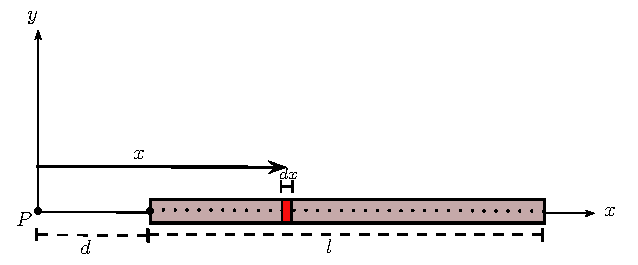
\includegraphics[scale=0.8]{gravitacion/barra1}
\end{center}
\caption{Campo en el eje de una barra de longitud $l$.}
\label{fig:gravitacion-barra1}
\end{figure}

\begin{eqnarray}
\vec{g}=-G\int_m \dfrac{dm}{r^2}\hat{u}_r = -G\int_m \dfrac{dm}{x^2}(-\hat{i})\,.
\end{eqnarray}
Usando la función densidad lineal de masa:
\begin{displaymath}
\lambda=\dfrac{dm}{dx}=\dfrac{m}{l} \Rightarrow dm=\dfrac{m}{l}dx\,, 
\end{displaymath}
tenemos que:
\begin{equation}
\vec{g}= -G\int_d^{d+l} \dfrac{dm}{x^2}(-\hat{i})=G \dfrac{M}{d(d+l)}\hat{i}\,.
\end{equation}

\item Una barra delgada de longitud $l$ tiene una masa $m$ uniformemente distribuida tal como se muestra en la Fig.~\ref{fig:gravitacion-barra2}. El campo en el punto $P$ está dado por:
\begin{figure}[h]
\begin{center}
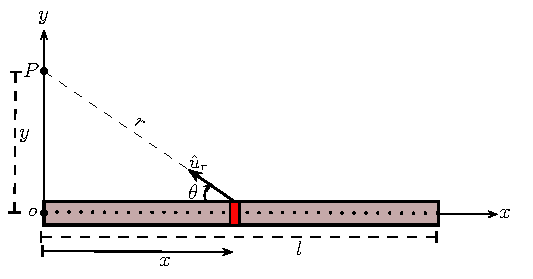
\includegraphics[scale=0.9]{gravitacion/barra2}
\end{center}
\caption{Campo en el eje perpendicular a un extremo de una barra de longitud $l$.}
\label{fig:gravitacion-barra2}
\end{figure}
\begin{eqnarray}
\nonumber \vec{g} & = & -G\int_m \dfrac{dm}{r^2}\hat{u}_r =-G\int_m \dfrac{dm}{r^2} (-\cos\theta \hat{i} + \sin\theta \hat{j})  \\ \nonumber
& = &-G\int_m \dfrac{dm}{r^2} (-\dfrac{x}{r} \hat{i} + \dfrac{y}{r} \hat{j}) 
=-G\int_0^l (m/l)dx(-\dfrac{x}{r^3} \hat{i} + \dfrac{y}{r^3} \hat{j}) \\\nonumber
&= &-\dfrac{Gm}{l}\int_0^l dx\Big(-\dfrac{x}{(y^2+x^2)^{3/2}} \hat{i} + \dfrac{y}{(y^2+x^2)^{3/2}} \hat{j}\Big) \\
&=& \dfrac{Gm}{l}\Big(\dfrac{1}{y}-\dfrac{1}{\sqrt{l^2+y^2}}\Big)\hat{i} -\dfrac{Gm}{y}\dfrac{1}{\sqrt{l^2+y^2}}\hat{j}\,.
\end{eqnarray}

\item Caso general: Campo en el punto $P$ mostrado en la Fig.~\ref{fig:gravitacion-barra3}.
\begin{figure}[h]
\begin{center}
\includegraphics[scale=1.2]{gravitacion/barra3}
\end{center}
\caption{Campo general a una distancia $y$ perpendicular al eje de una barra de longitud $l$.}
\label{fig:gravitacion-barra3}
\end{figure}
%
\begin{eqnarray}
\nonumber
\vec{g}&=&-G\int_m \dfrac{dm}{r^2}\hat{u}_r =-G\int_m \dfrac{dm}{r^2} (-\cos\theta \hat{i}+\sin\theta\hat{j}) = -G \lambda \int_m dx \bigg[\dfrac{-x}{r^3}\hat{i}+ \dfrac{y}{r^3}\hat{j}\bigg]\\ \nonumber
&=&-G \lambda \bigg[-\int_{-x_1}^{x_2}\dfrac{x dx}{(x^2+y^2)^{3/2}} \hat{i}+\int_{-x_1}^{x_2}\dfrac{ydx}{(x^2+y^2)^{3/2}}\hat{j}  \bigg] \\ 
&=&-G \lambda \Bigg[\bigg(\dfrac{1}{\sqrt{x_2^2+y^2} }-\dfrac{1}{\sqrt{x_1^2+y^2} } \bigg)\hat{i} + \dfrac{1}{y} \bigg(\dfrac{x_2}{\sqrt{x_2^2+y^2} }+\dfrac{x_1}{\sqrt{x_1^2+y^2} } \bigg)\hat{j} \ \Bigg] \,,
\end{eqnarray}
o alternativamente, usando $x_1=y/\tan\theta_1$ y $x_2=-y/\tan\theta_2$:
\begin{eqnarray}
\vec{g}=\dfrac{-G \lambda }{y}\bigg[(\sin\theta_1 -\sin\theta_2)\hat{i}+(\cos\theta_1 -\cos\theta_2)\hat{j}\bigg]\,.
\end{eqnarray}

En el caso de tener una \textit{barra infinita} de densidad $\lambda$ uniforme podemos usar el resultados anterior con $x_2 \rightarrow \infty$ y $x_1 \rightarrow \infty$ ó $\theta_1 \rightarrow 0$ y $\theta_2 \rightarrow \pi$, tal que:
%
\begin{eqnarray}
\vec{g}(y)=\dfrac{-2G\lambda}{y}\hat{j}\,.
\end{eqnarray}

\textbf{Ejercicio:} Use el resultado general para el campo de una barra y verifique los dos casos particulares hechos con anterioridad.

\end{enumerate}



\subsubsection{Campo de una anillo}
Un anillo de radio $R$ tiene una masa $m$ uniformemente distribuida. El campo $\vec{g}$ en un punto $P$ a lo largo del eje del anillo, tal como se muestra en la Fig.~\ref{fig:gravitacion-anillo}.
%
\begin{figure}[h]
\begin{center}
\includegraphics[scale=0.7]{gravitacion/anillo}
\end{center}
\caption{Campo en el eje de un anillo de radio R.}
\label{fig:gravitacion-anillo}
\end{figure}
%
\begin{eqnarray}
\nonumber \vec{g}
&=&-G\int_m \dfrac{dm}{r^2}\hat{u}_r =-G\int_m \dfrac{dm}{r^2}(\sin\theta \hat{k} - \cos\theta \hat{R}  )\\\nonumber
&=&-G\int_m \dfrac{dm}{r^2}[\sin\theta \hat{k} - \cos\theta (\cos\phi\hat{i}-\sin\phi\hat{j}) ] \\\nonumber
&=&-G\int_0^{2\pi} \dfrac{md\phi}{2\pi} \dfrac{1}{r^2}[\sin\theta \hat{k} - \cos\theta (\cos\phi\hat{i}-\sin\phi\hat{j}) ] \\
&=& -G \dfrac{m2\pi}{2\pi r^2}\sin\theta \hat{k}=-G \dfrac{m}{r^2}\left(\dfrac{z}{r}\right)\hat{k}=-Gm \dfrac{z}{(z^2+R^2)^{3/2}}\hat{k}\,.
\label{ec:campo-gravitacional-anillo}
\end{eqnarray}
Note que en el cálculo anterior usamos:
%
\begin{displaymath}
\lambda=\dfrac{m}{l}=\dfrac{m}{2\pi R}=\dfrac{dm}{dl}=\dfrac{dm}{Rd\phi}\Rightarrow dm=\dfrac{md\phi}{2\pi}\,.
\end{displaymath}


\subsubsection{Campo de una arandela y de un disco}
Considere un disco hueco de radio exterior $R_2$, radio interior $R_1$ y masa $m$ uniformemente distribuida. El campo gravitacional en el punto $P$ mostrado en la Fig.~\ref{fig:gravitacion-arandela} está dado por:
%
\begin{figure}[h]
\begin{center}
\includegraphics[scale=0.9]{gravitacion/arandela}
\end{center}
\caption{Arandela de radio interno $R_1$ y radio externo $R_2>R_1$.}
\label{fig:gravitacion-arandela}
\end{figure}
%
\begin{align}
\vec{g}=&\int_m G\dfrac{dm}{r^2}\hat{u}_r
= \int_m G\dfrac{\sigma\rho d\rho d\phi}{r^2}(\cos\theta \hat{k}-\sin\theta\hat{\rho})\nonumber\\
=& G\int_m\dfrac{\sigma\rho d\rho d\phi}{r^2}\left(\dfrac{z}{r} \hat{k}-\dfrac{\rho}{r} (\cos\phi \hat{i}+\sin\theta\hat{j})\right)
\nonumber\\
=& G\int_{0}^{2\pi}\int_{R_1}^{R_2}\dfrac{\sigma\rho d\rho d\phi}{(z^2+\rho^2)^{3/2}}\left(z \hat{k}-\rho (\cos\phi \hat{i}+\sin\theta\hat{j})\right)\nonumber\\
=& G\int_{R_1}^{R_2}\dfrac{2\pi\sigma\rho d\rho d\phi}{(z^2+\rho^2)^{3/2}} \hat{k}
=\dfrac{2mG}{(R_2^2-R_1^2)} \Bigg(\dfrac{z}{\sqrt{z^2+R_2^2} } - \dfrac{z}{\sqrt{z^2+R_1^2} }  \Bigg)\hat{k}\,.
\label{ec:campo-gravitacional-arandela}
\end{align}
%
Note que si $R_1 \rightarrow 0$, tenemos el campo de un disco o moneda de radio $R_2$:
%
\begin{equation}
\vec{g}(z)=\dfrac{-2mG}{R_2^2} \Bigg(1 - \dfrac{z}{\sqrt{z^2+R_2^2} }  \Bigg)\hat{k}\,.
\label{ec:campo-gravitacional-disco}
\end{equation}
Además, si $R_1 \rightarrow 0$ y $z >> R_2$ tenemos aproximadamente el campo de masa puntual $m$, lo cual es de esperarse ya que desde muy lejos cualquier configuración de masa ha de verse como una masa puntual, tal que:
%
\begin{equation}
\vec{g} \approx -G\dfrac{m}{z^2}\hat{k}\,.
\end{equation}  


\subsubsection{Campo de un plano}
%
\begin{figure}[h]
\begin{center}
\includegraphics[scale=0.6]{gravitacion/plano}
\end{center}
\caption{Plano infinito con densidad superficial de masa $\sigma$.}
\label{fig:gravitacion-plano}
\end{figure}
%
Para calcular el campo de un plano muy grande (infinito) con densidad de masa $\sigma$ uniforme podemos usar el resultado obtenido para el campo de disco dado por la ec.~\ref{ec:campo-gravitacional-disco}. El campo gravitacional del plano se obtiene haciendo infinito el radio del disco, tal como se muestra en la Fig.~\ref{fig:gravitacion-plano}. Es decir:
\begin{align}
\vec{g}=& \lim_{R\to\infty}\dfrac{-2mG}{R^2} \left(1 - \dfrac{z}{\sqrt{z^2+R^2} }  \right)\hat{k} 
= \lim_{R\to\infty}-2\pi\sigma G \left(1 - \dfrac{z}{\sqrt{z^2+R^2} }  \right)\hat{k}\nonumber\\
=& -2\pi\sigma G\, \hat{k}\,,
\label{ec:campo-gravitacional-plano}
\end{align}
donde usamos la función densidad $\sigma=m/(\pi R^2)$.



\subsubsection{Campo de una superficie esférica}
%
\begin{figure}[h]
\begin{center}
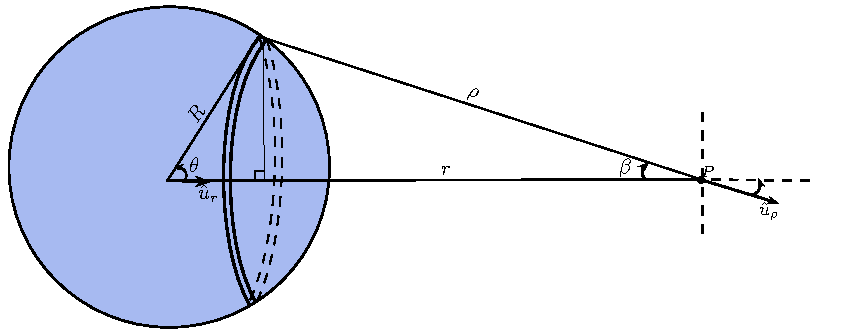
\includegraphics[scale=0.9]{gravitacion/esfera1}
\end{center}
\caption{Cascarón esférico de radio R.}
\label{fig:gravitacion-esfera}
\end{figure}
%
Calculemos el campo para un cascarón esférico de radio $R$ y masa $m$ uniformemente distribuida tal como se muestra en la Fig~\ref{fig:gravitacion-esfera}.

\begin{enumerate}
\item Para $r > R$ (exterior del cascarón esférico). De acuerdo a la Fig.~\ref{fig:gravitacion-esfera}:
\begin{eqnarray}
\vec{g}_p=-G\int_m \dfrac{dm}{\rho^2}\hat{u}_{\rho}\,.
\end{eqnarray}
Dada la simetría del problema, al integrar sólo sobrevive la componente del vector $\hat{u}_{\rho}$ en la dirección de $\hat{u}_r$, tal que:
\begin{eqnarray}
\vec{g}=-G\int_m \dfrac{dm}{\rho^2}\hat{u}_{\rho}==-G\int_m \dfrac{dm}{\rho^2} \cos\beta\, \hat{u}_r\,.
\end{eqnarray}
Además, si la distribución superficial de masa $\sigma$ es uniforme, entonces:
\begin{equation}
\sigma=\dfrac{m}{4\pi R^2}=\dfrac{dm}{dA}=\dfrac{dm}{2\pi R^2\sin\theta d\theta} \Rightarrow dm=\dfrac{1}{2}m\sin\theta d\theta ,
\end{equation}
Por otro lado, usando la ley del coseno en el triángulo de lados $r$, $R$ y $\rho$, tenemos:
%
\begin{equation}
\rho^2 =R^2 + r^2 -2Rr\cos\theta.  \hspace{0.5 cm} \text{Derivando} \Rightarrow \sin\theta d\theta = \dfrac{\rho}{Rr} d\rho\,.
\end{equation}
\begin{equation}
R^2=r^2+\rho^2 -2r\rho \cos\beta \Rightarrow \cos\beta =\dfrac{r^2+\rho^2 -R^2}{2r\rho}\,.
\end{equation}
%
Reemplazando las tres ecuaciones anteriores en la ecuación para el campo tenemos que:
\begin{eqnarray}
\vec{g}(r) &=& -\dfrac{Gm}{4Rr^2}\hat{u}_r \int_{r-R}^{r+R} \bigg(1+ \dfrac{r^2-R^2}{\rho^2}  \bigg)d\rho = -G \dfrac{m}{r^2}\hat{u}_r\,.
\label{ec:campo-gravitacional-cascaron}
\end{eqnarray}

\item Para $r < R$ (interior del cascarón esférico). De acuerdo a la Fig.~\ref{fig:gravitacion-esfera}:
\begin{eqnarray}
\vec{g} &=& -\dfrac{Gm}{4Rr^2}\hat{u}_r \int_{R-r}^{r+R} \bigg(1+ \dfrac{r^2-R^2}{\rho^2}  \bigg)d\rho = \hat{0}\,.
\end{eqnarray}
\end{enumerate}

El resultado obtenido para el campo gravitacional de un cascarón esférico, marca uno de los resultados fundamentales en la teoría de campo gravitacional. 
\begin{itemize}
\item El campo gravitacional en el exterior de un cascarón esférico, es equivalente al campo generado por una masa puntual $m$ situada en el centro de masa de dicho cascarón.
\item El campo gravitacional en el interior es nulo. 
\end{itemize}


\subsubsection{Campo de una esfera maciza con densidad de masa uniforme $\rho$}
%
\begin{figure}[h]
\begin{center}
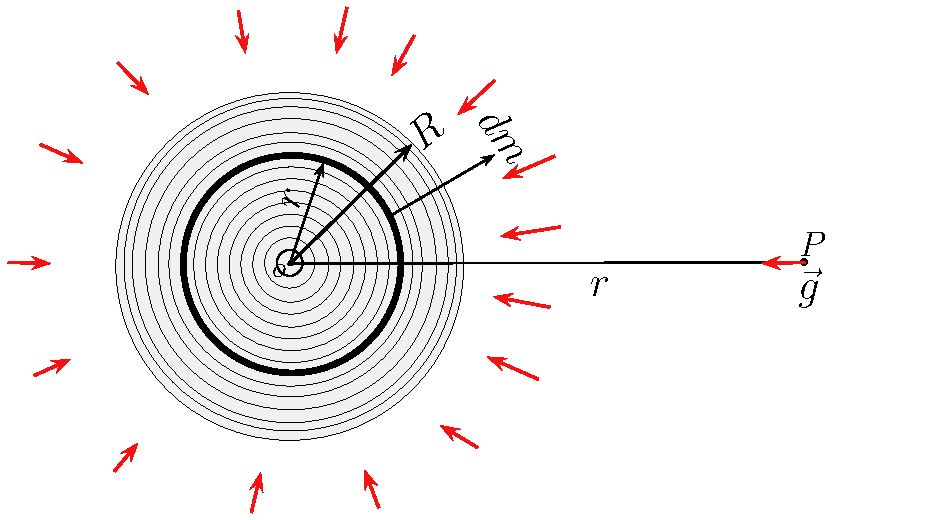
\includegraphics[scale=0.7]{gravitacion/esfera2}
\end{center}
\caption{Esfera maciza de radio $R$ y masa $m$.}
\label{fig:gravitacion-esfera2}
\end{figure}
%
\begin{enumerate}
\item Para $r > R$ (exterior de la esfera), podemos integrar en cascarones esféricos y usar el resultado obtenido para el campo generado por un cascarón de masa diferencial $dm$ en el punto $P$ (ec.~\eqref{ec:campo-gravitacional-cascaron}).
\begin{eqnarray}
\vec{g}(r)=\int_m d \vec{g} = \int_m \bigg(-G \dfrac{dm}{r^2}\hat{u}_r \bigg)=-G \dfrac{1}{r^2}\hat{u}_r\int_m dm= -G \dfrac{m}{r^2}\hat{u}_r\,,
\label{ec:campo-gravitacional-esfera-exterior}
\end{eqnarray}
donde debe quedar claro que ahora $m$ es la masa neta de la esfera maciza.

\item Para $r < R$ (interior de la esfera) sólo contribuye la masa $m'$ localizada en la esfera de radio $r < R$ tal como se muestra en la Fig.~\ref{fig:gravitacion-esfera2} , tal que:
\begin{eqnarray}
\vec{g}(r)=-G \dfrac{m'}{r^2}\hat{u}_r = -G \bigg(m \dfrac{r^3}{R^3} \bigg)\dfrac{1}{r^2}\hat{u}_r= -Gm \dfrac{r}{R^3}\hat{u}_r\,,
\label{ec:campo-gravitacional-esfera-interior}
\end{eqnarray}

donde tuvimos en cuenta que la densidad de la esfera es uniforme, así:
\begin{displaymath}
\rho=\dfrac{m}{\dfrac{4}{3}\pi R^3 } = \dfrac{m'}{\dfrac{4}{3}\pi r^3 } \Rightarrow m'=m \dfrac{r^3}{R^3}\,.
\end{displaymath}

\end{enumerate}

Al igual que el resultado obtenido para el campo gravitacional de un cascarón esférico. El campo de una esfera maciza marca uno de los resultados fundamentales en la teoría de campos. 
\begin{itemize}
\item El campo gravitacional atractivo en el exterior de una esfera, es equivalente al campo generado por una masa puntual $m$ situada en el centro de masa de la esfera. Note que externamente no importa si la masa $m$ está distribuida en un cascarón esférico o en una esfera maciza.
\item El campo gravitacional en el interior, es el campo generado por la masa localizada en una esfera de radio $r < R$, es decir, el campo es generado por la masa que hay desde el punto interno hasta el centro de masa. 
\end{itemize}






\subsection{Ejemplos de potencial gravitacional}


\subsubsection{Potencial de una barra}
Consideremos la barra mostrada en la Fig.~\ref{fig:gravitacion-barra3} de masa $m$ y longitud $l$. El potencial gravitacional en el punto $P$ es:
\begin{align}
V=&-\int_m G\dfrac{dm}{r} = -\int_m G \dfrac{\lambda dx}{r}
=-G\int_{-x_1}^{x_2}\dfrac{\lambda dx}{\sqrt{y^2+x^2}}\nonumber\\
=& -G\lambda \left[\ln\left(\dfrac{\sqrt{x_2^2+y^2}}{y}+\dfrac{x_2}{y}\right)-\ln\left(\dfrac{\sqrt{x_1^2+y^2}}{y}-\dfrac{x_1}{y}\right)\right]\nonumber\\
=& -G\lambda \ln\left(\dfrac{\sqrt{x_2^2+y^2}+x_2}{\sqrt{x_1^2+y^2}-x_1}\right)\,,
\label{ec:potencial-gravitacinal-barra}
\end{align}
donde $\lambda=m/l=m/(x_1+x_2)$ es la densidad de masa de la barra.

%Para el caso de un alambre muy largo (infinito) hacemos $x_1\to\infty$ and $x_2\to\infty$.



\subsubsection{Potencial de un anillo}

Consideremos el anillo de masa $m$ uniformemente distribuida y radio $R$ mostrado en la Fig.~\ref{fig:gravitacion-anillo}. El potencial gravitacional en el punto $P$ es:

\begin{eqnarray}
V=-G\int_m \dfrac{dm}{r}=-G \dfrac{1}{r}\int_m dm =-G \dfrac{m}{r}=-G \dfrac{m}{\sqrt{z^2+R^2}}\,,
\label{ec:potencial-gravitacinal-anillo}
\end{eqnarray}
donde la distancia $r$ desde el diferencial al punto medida $P$ es constante.
Por otro lado, note que:
\begin{eqnarray}
\vec{g}(z)=-\vec{\nabla}V=-\hat{k}\dfrac{d}{dz}V(z)=-Gm \dfrac{z}{(z^2+R^2)^{3/2}} \hat{k}\,.
\end{eqnarray}
Resultado idéntico al obtenido usando la definición de campo (ver ec.~\ref{ec:campo-gravitacional-anillo}). Tenga en cuenta que para este caso particular, ha sido más fácil calcular el potencial y a partir de él calcular el campo gravitacional. 

\textbf{Ejercicio:} Suponga que una masa $m'$ es colocada en el punto $P$. Calcule la rapidez de $m'$ justo cuando pasa por el centro del anillo. ¿Qué condición matemática debe cumplirse para que $m'$ ejecute un movimiento armónico simple? Determine la frecuencia de oscilación.\\
\textit{Respuesta:} 
\begin{displaymath}
v_0=\sqrt{2Gm( \dfrac{1}{R}-\dfrac{1}{\sqrt{R^2+z^2} } )}
\end{displaymath}
Si $z<<R \Rightarrow \dfrac{d^2z}{dt^2}+ \dfrac{Gm}{R^3} z \approx 0$ y así:
\begin{displaymath}
\omega_0=\sqrt{\dfrac{Gm}{R^3} }\,.
\end{displaymath} 



\subsubsection{Potencial de una arandela y un disco}
Calculemos el potencial gravitacional de la arandela de radio exterior $R_2$ y radio interior $R_1<R_2$ en el punto $P$ mostrado en la Fig.~\ref{fig:gravitacion-arandela}.
\begin{align}
V=& -G\int_m \dfrac{dm}{r} = -G\int_0^{2\pi}\int_{R_1}^{R_2}\dfrac{\sigma \rho d\rho d\phi}{\sqrt{z^2+\rho^2}}\nonumber\\
=& -G\int_{R_1}^{R_2}\dfrac{\sigma 2\pi\rho d\rho }{\sqrt{z^2+\rho^2}}=-2\pi\sigma G\left(\sqrt{R_2^2+z^2} -\sqrt{R_1^2+z^2}\right)
\nonumber\\
=& -\dfrac{2G m}{(R_2^2-R_1^2)} \left(\sqrt{R_2^2+z^2} -\sqrt{R_1^2+z^2}\right)\,.
\label{ec:potencial-gravitacional-arandela}
\end{align}
Note que podemos determinar el campo gravitacional a partir de este potencial de la siguiente manera:
\begin{align}
\vec{g}(z)=&-\vec{\nabla}V(z)=-\hat{k}\dfrac{d}{dz}V(z)\nonumber\\
=&\dfrac{2mG}{(R_2^2-R_1^2)} \Bigg(\dfrac{z}{\sqrt{z^2+R_2^2} } - \dfrac{z}{\sqrt{z^2+R_1^2} }  \Bigg)\hat{k}\,,
\end{align}
expresión que fue calculada directamente con la definición del campo gravitacional (ver ec.~\ref{ec:campo-gravitacional-arandela}).

Para un disco de radio $R$ y masa $m$ usamos la ec.~\ref{ec:potencial-gravitacional-arandela} con $R_1=0$ y $R_2=R$, tal que:
\begin{align}
V=& -\dfrac{2G m}{R^2} \left(\sqrt{R^2+z^2} -z\right)=-2\pi G \sigma \left(\sqrt{R^2+z^2} -z\right)\,.
\label{ec:potencial-gravitacinal-disco}
\end{align}



\subsubsection{Potencial de un plano infinito con densidad superficial de masa $\sigma$ constante}

\begin{equation}
V(z)=\lim_{R\to\infty} V_{\text{disco}} 
=\lim_{R\to\infty} \left[-2\pi G \sigma \left(\sqrt{R^2+z^2} -z\right)\right] = -\infty +2\pi G \sigma z\,,
\end{equation}
dado que el potencial es infinito, realizamos el proceso de renormalización. Éste consiste en tomar la parte finita del potencial. Por lo tanto, el potencial renormalizado de un plano infinito de densidad de masas $\sigma$ es:
\begin{equation}
V(z)=2\pi G \sigma z\,.
\label{ec:potencial-gravitacional-plano}
\end{equation} 
Note que podemos determinar el campo gravitacional a partir de este potencial de la siguiente manera:
\begin{eqnarray}
\vec{g}=-\vec{\nabla}V(z)=-\hat{k}\dfrac{d}{dz}(2\pi G \sigma z)=-2\pi\sigma G \hat{k}\,,
\end{eqnarray}
el cual fue calculado directamente con la definición del campo gravitacional (ver ec.~\ref{ec:campo-gravitacional-plano}).



\subsubsection{Potencial de una superficie esférica de radio R} 

\begin{enumerate}
\item Para el exterior del cascarón esférico ($r \geq R$):

\begin{equation}
V=-G \dfrac{m}{r}  
\end{equation}

\item Para el interior del cascarón esférico ($r \leq R$):

\begin{equation}
V=-G \dfrac{m}{R}=cte.
\end{equation}

\end{enumerate}

\subsubsection{Potencial de una esfera maciza de radio R}

\begin{enumerate}
\item Para el exterior de la esfera ($r \geq R$):

\begin{equation}
V=-G \dfrac{m}{r}  
\end{equation}

\item Para el interior de la esfera ($r \leq R$):

\begin{equation}
V=\dfrac{Gm}{2R^3}(r^2-3R^2)
\end{equation}

\end{enumerate}
%%%%%%%%%%%%%%%%%%%% END GRAV %%%%%%%%%%%%%%%%%%%%%%%%%%%%%%